\documentclass[12pt,a4paper,twoside,openright]{book}

\usepackage{hyperref}
\usepackage[english]{babel}
\usepackage{style/isi-lm}
\usepackage{cleveref}
\usepackage{subcaption}

\definecolor{dkgreen}{rgb}{0,0.6,0}
\definecolor{gray}{rgb}{0.5,0.5,0.5}
\definecolor{mauve}{rgb}{0.58,0,0.82}

\lstset{
  frame=single,
  captionpos=b,
  language=Java,
  aboveskip=3mm,
  belowskip=3mm,
  showstringspaces=false,
  columns=flexible,
  basicstyle={\small\ttfamily},
  numbers=left,
  numberstyle=\tiny\color{gray},
  keywordstyle=\color{blue},
  commentstyle=\color{dkgreen},
  stringstyle=\color{mauve},
  breaklines=true,
  breakatwhitespace=true,
  tabsize=2
}

\lstdefinelanguage{TypeScript}{
  keywords={undefined, typeof, new, true, false, catch, function, return, null, catch, switch, var, if, in, while, do, else, case, break, export, const, string, this},
  ndkeywords={},
  sensitive=false,
  comment=[l]{//},
  morecomment=[s]{/*}{*/},
  morestring=[b]',
  morestring=[b]",
  breaklines=true,
  breakatwhitespace=true,
  columns=flexible
}

\lstdefinelanguage{Turtle}{
  keywords={workspaces, 102, type, WorkspaceArtifact, Workspace, Thing, directlyContains, hypermedia_body_1, hypermedia_body_2, hasActionAffordance}
}



%--------------------------------------------------------------------
%---------------------- INFORMAZIONI SULLA TESI ---------------------
%--------------------------------------------------------------------

\universita{Alma Mater Studiorum -- Università di Bologna}
\campus{Campus of Cesena}
\dipartimento{Computer Science and Engineering Department}
\cdl{Second Cycle Degree in Computer Science and Engineering}

\titolo{Visual Programming Paradigm for Hypermedia Multi-Agent Systems}
\materia{Pervasive Computing}

\laureando{Alessandro Marcantoni}

\relatore[Prof.]{Alessandro Ricci}
\correlatorea[Prof.]{Simon Mayer}
\correlatoreb[Dott.]{Samuele Burattini}

\annoaccademico{2021 -- 2022}

\parolechiave{Multi-Agent Systems}{Visual Programming}{Organization}{Hypermedia}{Web IDE}

\dedica{To the ones who have always believed in me}

\makeindex

\begin{document}
\frontmatter
\maketitle
\tableofcontents

\chapter{Introduction}
\markboth{INTRODUCTION}{INTRODUCTION}

Qui il testo dell'introduzione alla tesi. Generalmente l'introduzione non dovrebbe superare le 2/3 pagine e dovrebbe essere scritta solo alla fine.
	
\mainmatter

\pagestyle{fancy} 
\fancyhead[LE,RO]{\thepage}
\fancyfoot{}

\chapter{Context, Motivations and Research Proposal}\label{context}
This project was born thanks to the collaboration between the \textit{Pervasive Software Lab}\footnote{\href{https://apice.unibo.it/xwiki/bin/view/PSLab/}{https://apice.unibo.it/xwiki/bin/view/PSLab/}} of the \textit{University of Bologna} and the \textit{Interaction- and Communication-based Systems}\footnote{\href{https://ics.unisg.ch/chair-interactions-mayer/}{https://ics.unisg.ch/chair-interactions-mayer/}} research group of the \textit{University of St.\ Gallen}, in Switzerland.

Since both groups are interested and involved in similar research topics, such as the interactions among devices and people in ubiquitous computing environments, a highly enriching opportunity for an internship abroad arose.

Moreover, the research group in St.\ Gallen is contributing to a European project named \textit{IntellIoT}\footnote{\href{https://intelliot.eu/}{https://intelliot.eu/}}, which stands for ``Intelligent IoT'' and whose aim is, together with its partners, to develop a reference architecture to enable IoT environments for semi-autonomous IoT applications endowed with intelligence that evolves with the Human-in-the-Loop.
Hence, the concurring perspective of the two research groups and the St.\ Gallen group's participation in such a visionary initiative made it easy to shape the requirements of the thesis work.

The following sections will present the main objectives of the \textit{IntellIoT} project to describe the context in which the thesis was conducted.

% Description of the other sections.
\newpage

\section{The \textit{IntellIoT} Project}\label{intelliot-project}
\textit{IntellIoT} is a Pan-European project that focuses on developing integrated, distributed, human-centered and trustworthy IoT frameworks, with particular attention to sectors like agriculture, healthcare, manufacturing, energy, construction, and smart cities.

To achieve the latter goals, \textit{IntellIoT} explores and exploits new enabling technologies such as 5G connectivity, distributed technology, Augmented Reality, Artificial Intelligence, and tactile internet.
Of course, this is possible thanks to the project's partners spread across ten countries that form a competitive ecosystem.

Among them, the \textit{University of St.\ Gallen} is currently focusing on integrating physical things into the Web, increasing the autonomy of Web-enabled devices, and making interactions of connected devices intelligible for people using \textbf{Hypermedia Multi-Agent Systems}.
Indeed, the primary objective of this thesis is to explore how humans can effectively define such systems' organization.

\subsection{Mission}
Smart technologies play a significant role in our life and work.
However, the traditional approach based on cloud technologies has limitations, such as unreliable connectivity, limited bandwidth, long reaction times, lack of autonomy, and trust concerns.
Therefore, the goal of \textit{IntellIoT} is to tackle these issues and create a framework enabling next-generation IoT solutions. Specifically, these issues are addressed by focusing on the following three pillars, which are the central research topics of the project.

\subsubsection{Collaborative IoT}
Various semi-autonomous entities should cooperate to achieve the system's overall goal.
Hence, self-awareness and knowledge of the task to perform and the environment where they are located are vital abilities to seek.
Entities can acquire knowledge either by interacting with the environment via sensors or by reliable and secure communication with each other.
However, since providing complete knowledge to entities in open and continuously changing environments is practically infeasible, Artificial Intelligence and Machine Learning come to the rescue.

\subsubsection{Human-in-the-Loop}
Since IoT applications cannot be completely autonomous in how they decide and act, humans need to be involved in controlling and optimizing the Artificial Intelligence the devices are endowed with.
Indeed, the interaction between humans and intelligent systems can expand the latter's knowledge about the environment or the application by exploiting the former's experience.
In fact, by applying Machine Learning algorithms, the devices can learn new features and information about the overall process so that they will have enough knowledge to react to similar scenarios in the future automatically.

\subsubsection{Trustworthiness}
As beneficial as IoT devices are, they present some major security concerns.
The Mirai botnet exploiting embedded devices to perform DDoS attacks \cite{antonakakis2017understanding}, possibly hackable cardiac devices, and Stuxnet sabotaging Iranian nuclear facilities \cite{baezner2017stuxnet} are only a few examples of critical breaches.
Thus, security, privacy, and trust are vital for IoT systems and applications and their broader acceptance.
Therefore, these concepts must be considered early in the design process and regard computation and communication infrastructure.

\begin{figure}[H]
    \centering
    \includegraphics[width=0.8\linewidth]{images/intelliot-pillars.png}
    \caption{The three pillars of \textit{IntellIoT}.}
    \label{fig:intelliot-pillars}
\end{figure}

\subsection{Use Cases}
The above three key component areas are supported by \textit{IntellIoT}'s dynamically managed network and computation infrastructure that, combined, provide resource and edge management, orchestration capabilities, and network choreography, exploiting cutting-edge technologies like 5G.
Moreover, for the pillars to not remain only abstract concepts, various use cases that aim to address real-life problems in three core sectors were developed:

\begin{itemize}
    \item \textbf{Agriculture}: the application of IoT in agriculture could be a life-changer for humanity as we now witness how extreme weather, deteriorating soil, dry lands, and collapsing ecosystems make food production more and more complicated and expensive, not to mention the population growth that increases the demand for resources.
    Although ``smart farming'' is already a thing, \textit{IntellIoT} aims to bring it to the next level thanks to autonomous devices such as self-driving tractors and drones endowed with sensors and actuators.
    However, even though machines perform potentially dangerous, tiring, and repetitive tasks for humans, the latter still play a crucial role in managing the farm.
    Indeed, they can remote control the devices in uncertain situations, refining the Artificial Intelligence models.
    Additionally, human operators are in charge of defining the goals of the farming system, leveraging their experience and knowledge about the domain.
    \item \textbf{Healthcare}: IoT is revolutionizing the healthcare industry, mainly due to remote patient monitoring.
    Indeed, being endowed with specific sensors, devices can track the latter's vital signs and other health metrics and send the collected data to healthcare providers.
    Some examples of such devices are \textit{Continuous Glucose Monitoring} \cite{facchinetti2013real} and \textit{Dissolvable Brain Swelling}\cite{kang2016bioresorbable} sensors or ordinary smartwatches.
    This process improves the patient's quality of life, which does not need to be limited to their home or the hospital and can thus carry on with their regular everyday activities.
    Moreover, continuous monitoring and real-time data sharing allow timely interventions when necessary, and automatic data collection can drastically decrease the time and effort required to retrieve and manage information about the patient.
    Not to mention the opportunities for data analysis and possible Artificial Intelligence models that would support clinicians in being more efficient.
    However, this workflow potentially exposes patients' sensitive information; therefore, we find privacy, security, and trust assurance among the main focuses of \textit{IntellIoT} regarding this use case.
    \newline
    \item \textbf{Manufacturing}: IoT is one of the core driving forces behind Industry 4.0, which aims to digitalize and automate operational processes counting on as little support as possible from human operators, from the order submission to the delivery of the product.
    Leveraging AI and Machine Learning, robotics, and data analysis, IntellIoT envisions a future with shared manufacturing plants and multiple customers utilizing manufacturing as-a-service.
    According to the latter scenario, an intelligent IoT environment would derive a production plan from data received from a customer and select the appropriate machines for the planned steps.
    However, whenever AI is not sufficiently confident about a step, a human-in-the-loop can take over control remotely, providing information that will be learned by the Machine Learning algorithm thanks to continual learning.
\end{itemize}

\section{Domain-Expert Programming}
As already discussed, the crucial role of end-users in the definition of autonomous systems, the importance of their intervention in case of need, and their expertise are utterly unmatched by Artificial Intelligence algorithms and probably will be for a long time.

On top of that, the gap between programmers and end-users regarding domain comprehension is a well-acknowledged issue concerning software development.
Indeed, developers' poor understanding of the domain often results in projects missing their schedules or exceeding their budget, poor-quality software, or even wrong functionalities \cite{5089292}.
To address this critical issue, several techniques have been developed.
For instance, one of the core aspects of Domain Driven Design is \textit{knowledge crunching}, which aims to extract domain knowledge from the experts to reflect it in the code during the subsequent development phases.

On the other hand, a different approach might be taken directly involving domain experts in the programming process.
This kind of user can be defined as professionals in some domain different from computer science who need to use computers in their daily work and often have real needs to perform some programming activities that result in the creation or modification of software artifacts \cite{costabile2003domain}.
Given the latter definition and the premise suggesting the importance of domain expertise, providing domain experts with tools, such as domain-specific languages (DSL) or more user-friendly visual tools, that allow them to ``code'' or configure parts of complex systems feels very natural.
Therefore the need for an intuitive development environment in which users with no proper computer science background can naturally and seamlessly transform their domain knowledge into specifications with low-code (or possibly no-code).

\section{Visual Programming Paradigm}
Multi-Agent Systems is one of the core enabling technologies of the infrastructure of \textit{IntellIoT}.
MAS fit IoT because they tackle the complexity and handle the decentralization of the IoT ecosystem by providing a framework for coordinating the actions of a large number of devices, allowing the latter to communicate and make decisions toward the achievement of a common goal.
Another critical advantage of MAS is their ability to deal with partial knowledge, incomplete and imperfect information, and adapt and reason in real-time, which is crucial in dynamic, uncertain, open, and distributed networks.

However, the high-level expertise required to program agent-based systems hinders the large-scale adoption of MAS.

\subsection{Agent-Oriented Visual Programming}
To facilitate the spread of this technology, efforts have been made to eliminate the entry barrier to MAS development.
One example of such endeavor is the development of an agent-oriented programming paradigm \cite{burattini2022agent}, which enables individuals without coding experience, but with knowledge of specific target domains, to design and (re)configure autonomous software.

This proposal makes the development of software agents easier in two ways:
\begin{itemize}
    \item \textbf{Use of human-oriented abstractions}: the application of the BDI (Belief-Desire-Intention) model, which makes use of concepts such as goals, plans, beliefs, and intentions, allows defining the agent's behavior more naturally, as this paradigm matches more closely people's everyday experience.
    \item \textbf{Use of visual programming techniques}: this project makes use of block-based programming, which is a visual programming paradigm that uses blocks to represent the program's instructions.
    The adoption of a no-code environment allows non-technical users to easily create and modify agents.
\end{itemize}

\begin{figure}[H]
    \centering
    \includegraphics[width=0.8\linewidth]{images/blocks-example.png}
    \caption{Example of a ``ping'' agent implemented with the block language. Adopted from~\cite{burattini2022agent}.}
    \label{fig:blocks-example}
\end{figure}

An example of this work can be found in \cref{fig:blocks-example}, which shows a simple ``ping'' agent.
When started, the agent has a belief that the \texttt{wait\_time} is $2$ seconds, and it has to achieve the goal \texttt{ping}.
In addition, the agent is given instructions on how to achieve the goal through a plan.
The latter states that when the agent decides to achieve the goal \texttt{ping} and knows what the \texttt{wait\_time} is, it should first wait for the time specified in its belief, then send a message to the agent \texttt{pong}.

\subsection{Proposing a Visual Programming Paradigm for Organizations}
Although the above block-based visual development environment is suitable for defining single entities, a level of abstraction to handle the relations among and coordination of the latter is still missing.

When dealing with multiple agents in a MAS, the complexity of the system increases dramatically and the coordination of and interaction among the agents' becomes more and more challenging.
Even though these aspects could be technically represented and managed directly in the mind of the agents, the adoption of adequate abstractions makes the solution dramatically more straightforward and elegant. \cite{boissier2020multi}

Therefore, the idea is to design and implement a visual language and a supportive development environment for MAS organizations, which is a novelty to our knowledge.
The core thesis work will be based on studying the existing organization models, with particular attention to the \moiseplus{} model, and developing an appropriate representation that could provide a suitable tradeoff between the expressiveness of code-based specifications and the ease of use of graphic programming interfaces.
A qualitative evaluation is also planned to receive feedback for the developed framework and to study how non-technical users solve problems by exploiting the visual language.

The following chapter provides an introduction to the background of the main technologies and research topics explored in the project.
\chapter{Background}\label{background}
To better understand this thesis work, a brief excursus of the existing literature about the main concepts the project relies on is presented. The aim is to provide some basic knowledge of the topics to understand what is considered state-of-the-art and to introduce some of the technologies exploited to develop the project.

\section{Multi-Agent Systems}
Multi-Agent Systems are considered a promising engineering style for developing adaptive software systems able to handle the continuous increase in their complexity.
Moreover, they allow the design and implementation of software systems using the same ideas and concepts that are the very founding of human societies and habits.

In this section, a brief overview of the main concepts and characteristics of MAS is provided, as well as the main approaches to their design.

\subsection{What is an Agent?}
The concept of a software agent can be traced back to the early days of research into Distributed AI in the 1970s when Carl Hewitt proposed the concurrent Actor model.
In his paper, he introduced the concept of a self-contained, interactive, and concurrently-executing object which he termed ``actor''.
The latter is a computational \textit{agent} with a mail address and behavior.
Actors can communicate by message-passing and carry out their actions concurrently.~\cite{hewitt1977viewing}

Software agents strongly rely on many of the concepts introduced by the Actor model, such as the idea of a self-contained entity endowed with its control flow that can interact with other entities and the use of message-passing for communication.
On top of that, agents bring in autonomous and proactive behavior as researchers were interested in the development of systems made up of entities with human-like skills such as reasoning, problem-solving, and decision-making.

The term ``agent'' quickly spread to heterogeneous research fields; therefore, there is no commonly agreed definition for it.
However, a generally accepted description of what an agent is is the following by Wooldridge~\cite{490039}:
\begin{quote}
    \textit{An agent is a self-contained program capable of controlling its own decision-making and acting, based on its perception of its environment, in pursuit of one or more objectives.}
\end{quote}
To sum up, a set of features that an agent should possess can be identified~\cite{490039}:
\begin{itemize}
    \item \textbf{Autonomy}: agents should be able to perform most of their tasks without the direct intervention of humans or other agents, and they should encapsulate control over their actions and internal state
    \item \textbf{Social ability}: agents should be able to interact with each other and possibly humans to complete their tasks.
    \item \textbf{Responsiveness} (situatedness): agents should perceive their environment and respond to changes in it.
    \item \textbf{Proactiveness}: agents should exhibit opportunistic, goal-directed behavior and take the initiative when appropriate.
\end{itemize}

Since the first years, the research concentrated on interaction and communication among agents, decomposition and distribution of tasks, and coordination and cooperation.
The goal was to specify, analyze, design, and integrate systems containing multiple collaborative agents.

\subsection{From the Individual to the Collective}
Multi-Agent Systems (MAS) have been studied as a per se field since the 1980s and gained widespread recognition in the 1990s.
Since then, international interest in the topic has grown enormously as agents are considered an appropriate paradigm to exploit the possibilities presented by massive open distributed systems.
Moreover, MAS seem to be a natural metaphor for understanding and building a wide range of what might be called \textit{artificial social systems}.~\cite{wooldridge2009introduction}

According to the \textit{Alan Turing Institute}~\cite{turing}
\begin{quote}
    \textit{A Multi-Agent System consists of multiple decision-making agents which interact in a shared environment to achieve common or conflicting goals.}
\end{quote}

\begin{figure}
    \centering
    \includegraphics[width=0.9\linewidth]{images/multi-agent-systems.png}
    \caption{A representation of Multi-Agent Systems.~\cite{jennings2000agent}}
    \label{fig:multi-agent-systems}
\end{figure}
Therefore, as it can also be noticed in \cref{fig:multi-agent-systems}, MAS are composed of an environment and agents existing within it that are bonded by relations.

\section{Multi-Agent Oriented Programming}
In principle, there is no constraint on the programming technologies that can be used to implement MAS.
However, the risk is to have an agent-centered interpretation of the system in which the environment and/or the organization contexts are represented and managed in the mind of the agents.
Therefore, the adoption of programming languages and paradigms that directly support first-class abstractions for these contexts highly simplifies the task of designing and implementing MAS and makes it possible to keep the level of abstraction coherent from design time to development time and finally also at runtime.

\textit{Multi-Agent Oriented Programming} (MAOP) is an approach to programming MAS that promotes the use of first-class programming abstractions that concern three main dimensions that characterize these systems:~\cite{boissier2020multi}
\begin{itemize}
    \item \textbf{Agent dimension}: it concerns the concepts and programming abstractions for the definition of the agents that participate in the system.
    Specifically, it allows the definition of software entities with their logical thread of control, which can autonomously and proactively achieve their goals, and interact with the environment, other agents, and the organization that regulates the system.
    \item \textbf{Environment dimension}: it offers concepts and abstractions to define the distributed resources and connections to the world shared among the agents.
    Thus, the environment abstraction is what makes the agents situated and provides them with tools that help them achieve their goals.
    \item \textbf{Organization dimension}: it collects all the concepts regarding the definition of relations, shared tasks, and policies among agents (inter)acting in a shared environment.
    In open systems, the organization is fundamental for coordination and regulation among agents.
\end{itemize}

Since agents have already been discussed, the following sections provide a description of the latter two dimensions, with a particular focus on the one regarding the organization, as it is the core of this thesis work.

\subsection{Environment in Multi-Agent Systems}
The environment in MAS plays a dual role~\cite{weyns2007environment}:
\begin{itemize}
    \item \textit{The ``external world''}:
    agents become aware of the context they are immersed in and its dynamics by perceiving the environment through sensors.
    Moreover, they pursue their goals through actions performed by actuators that aim at modifying the environment, eventually reaching the latter's desired state.
    \item \textit{A medium for coordination}:
    agents exploit the environment to share information and coordinate their behavior.
    Each agent follows simple behavioral rules, resulting in a collective behavior that is more complex than the sum of the individual behavior; this pattern resembles stigmergic systems in which agents coordinate their behavior through the manipulation of marks.
\end{itemize}
The environment not only enables the agents to interact with the deployment context, which they can access through sensors and actuators but also provides them with external resources that they can exploit to achieve their goal.

The \textit{Agents \& Artifacts} (A\&A) conceptual framework~\cite{ricci2007artifacts} argues that, just like in human society, MAS environments should contain different kinds of objects, tools, and artifacts in general that agents can use to support their activities.
This vision also constitutes a revolution from an engineering perspective as it encourages system designers to model the environment as a set of \textit{artifacts}, each of which encapsulates its intended purpose and exposes its observable state.
Moreover, the A\&A meta-model provides an effective abstraction level that shields low-level details of the deployment context, so that designers can focus on the agents' behavior.

\subsection{Organization in Multi-Agent Systems}
An agent organization can be defined as a social entity composed of a specific number of agents that accomplish several common tasks or goals and that are structured following some specific topology and communication interrelationships to achieve the main aim of the organization.
All MAS possess some form of organization, although it may be implicit and informal.

\subsubsection{Approaches to Organization in MAS}
There are two approaches to organizing agents in a MAS.~\cite{Ahmed_Abbas_2015}
The first one regards \textit{agent-centered} MAS, in which the focus is given to individual agents.
According to this viewpoint, the designer should concern about the local behavior of the agents and their interactions without worrying about the global structure and goal of the system as the latter should emerge as a result of the lower-level individual interactions in a bottom-up fashion.
The key issues of this approach are unpredictability and uncertainty since it could lead to undesirable emergent behaviors.
As Weyns~\cite{weyns2010organizations} stated, giving the responsibility of system organization implicitly to individual agents is highly complex and not suitable for real-world large-scale scenarios.

The second approach is \textit{organization-centered} MAS, in which the structure of the system is given greater attention.
The developer designs the entire organization and coordination patterns on the one hand, and the agents' local behavior on the other.
This can be seen as a top-down approach as the organization abstractions impose constraints on the agents and regulate their interactions, simplifying the design of complex and scalable systems and allowing more accurate modeling of the problems being tackled.
On top of that, the organization-centered approach avoids the emergence of undesirable behaviors such as divergence.
Indeed, larger MAS bring a higher risk of divergence, therefore the need for explicit organizational regulation.

\subsubsection{Organizational Paradigms}
Although no two organizational instances are likely to be identical, there are identifiable classes of organizations, that emerged from research and real-world applications, which share common characteristics.
These classes are called \textit{organizational paradigms} and cover particularly common, useful, or interesting structures that can be described in some general form.
Here is provided a brief overview of the most common paradigms~\cite{horling_lesser_2004}:
\begin{itemize}
    \item \textbf{Hierarchies}: agents are conceptually arranged in a tree-like structure, where agents higher in the tree have a more global view than those below them.
    Interactions only take place between connected entities; data produced by lower-level agents in a hierarchy typically travels upwards to provide a broader view, while control flows downwards as the higher-level agents provide directions to those below.
    \item \textbf{Holarchies}: agents are organized in holons.
    The term \textit{holon} comes from the Greek words \textit{holos}, meaning ``whole'', and \textit{on}, meaning ``part''. Therefore, a holon is a self-contained entity that can be considered both as a part of a larger entity and as a whole in itself, and that has a character derived but distinct from the entities that make it up and at the same time it contributes to the properties of a greater whole.
    Examples showed how holarchies can be used to effectively model the division of labor in MAS, where capabilities and tasks were imparted to holons instead of single agents.
    This results in a layer of abstraction that allows other entities to interact with a group as a single functional unit.
    \item \textbf{Coalitions}: they are formed by agents that share a common goal and that are willing to cooperate to achieve it and are generally short-lived as they are formed with a purpose in mind and dissolved when that need no longer exists.
    Although there may be a distinguished ``leading agent'', within a coalition the structure is typically flat.
    However, since once formed coalitions may be treated as a single entity, it is possible to form a hierarchical structure by nesting coalitions.
    \item \textbf{Teams}: they consist of several cooperative agents that agreed to work together towards a common goal.
    Unlike coalitions, teams attempt to maximize the performance of the group as a whole, rather than the performance of individual agents.
    This is usually achieved by assigning roles to the agents, which become responsible for specific tasks, and by providing the agents with representations of the shared goals, knowledge, and plans.
    \item \textbf{Congregations}: although similar to the latter two structures, they differentiate because they are assumed to be long-lived and are not necessarily formed with a specific goal in mind.
    Indeed, congregations are formed among agents with similar o complementary characteristics to facilitate the process of finding partners for collaborations.
    \item \textbf{Societies}: they are open systems where agents of different kinds may come and go at will while the society persists, acting as an environment through which the participants meet and interact.
    Societies impose on agents a set of constraints which are known as \textit{social laws}, \textit{norms}, or \textit{conventions}.
    These represent rules by which agents must act and provide a level of consistency in behavior that facilitates the coexistence of possibly heterogeneous agents.
    \item \textbf{Federations}: they are groups of agents which have ceded some amount of autonomy to a single delegate who represents the group.
    The members of the group interact only with the delegate, who accepts skills and needs descriptions from them, which are then used to match with requests from delegates representing other groups.
    \item \textbf{Markets}: buying agents may request or place bids for a common set of items, such as shared resources, tasks, services, or goods, or even supply items to the markets to be sold.
    On the other hand, sellers are responsible for processing bids and determining the winner.
    \item \textbf{Matrix}: they can be seen as a relaxation of the one-agent, one-manager restriction in hierarchical organizations, that permit many managers to influence the activities of an agent.
\end{itemize}

\begin{figure}
    \begin{subfigure}[h]{0.3\linewidth}
        \includegraphics[width=\textwidth]{images/orgs/org-hierarchy.png}
        \caption{Hierarchiy}
        \label{fig:hierarchy}
    \end{subfigure}
    \begin{subfigure}[h]{0.3\linewidth}
        \includegraphics[width=\textwidth]{images/orgs/org-holarchy.png}
        \caption{Holarchy}
        \label{fig:holarchy}
    \end{subfigure}
    \begin{subfigure}[h]{0.3\linewidth}
        \includegraphics[width=\textwidth]{images/orgs/org-coalitions.png}
        \caption{Coalitions}
        \label{fig:coalitions}
    \end{subfigure}
    \begin{subfigure}[h]{0.3\linewidth}
        \includegraphics[width=\textwidth]{images/orgs/org-teams.png}
        \caption{Team}
        \label{fig:teams}
    \end{subfigure}
    \begin{subfigure}[h]{0.25\linewidth}
        \includegraphics[width=\textwidth]{images/orgs/org-congregations.png}
        \caption{Congregations}
        \label{fig:congregations}
    \end{subfigure}
    \begin{subfigure}[h]{0.3\linewidth}
        \includegraphics[width=\textwidth]{images/orgs/org-societies.png}
        \caption{Society}
        \label{fig:societies}
    \end{subfigure}
    \begin{subfigure}[h]{0.3\linewidth}
        \includegraphics[width=\textwidth]{images/orgs/org-federations.png}
        \caption{Federations}
        \label{fig:federations}
    \end{subfigure}
    \begin{subfigure}[h]{0.3\linewidth}
        \includegraphics[width=\textwidth]{images/orgs/org-markets.png}
        \caption{Markets}
        \label{fig:markets}
    \end{subfigure}
    \begin{subfigure}[h]{0.3\linewidth}
        \includegraphics[width=\textwidth]{images/orgs/org-matrix.png}
        \caption{Matrix}
        \label{fig:matrix}
    \end{subfigure}
    \caption{Visual representation of the organizational paradigms.}
    \label{fig:organizational-paradigms}
\end{figure}

All of the above structures come with their benefits and drawbacks
%, which are briefly summarized in~\cref{table:orgs-advantages-disadvantages}
and it is generally agreed that there is no single type of organization that is suitable for all situations.
Indeed, sometimes two or more organizational paradigms may be combined to form a compound organization, exploiting features of each of the component organizations.


% \begin{table}[h]
%     \centering
%     \begin{tabular}{ | l p{0.4\linewidth} p{0.4\linewidth} | }
%         \hline
%         \textbf{Paradigm} & \textbf{Benefits} & \textbf{Drawbacks} \\\hline\hline
%         Hierarchy & Maps to many common domains; handles scale well & Potentially brittle; can lead to bottlenecks \\\hline
%         Holarchy & Exploit autonomy of functional units & Must organize holons, lack of predictable performance. \\\hline
%         Coalition & Exploit strength in number & Individual goals are preferred to common goals \\\hline
%         Team & Address larger problems; task-centric & Increased communication \\\hline
%         Congregation & Facilitates agents discovery & Sets may be overly restrictive \\\hline
%         Society & Public services; well-defined conventions & Potentially complex; agents may require society-related capabilities \\\hline
%         Federation & Matchmaking, brokering, and translation services facilitate dynamic agent pool & Intermediaries become bottlenecks \\\hline
%         Market & Good at allocation, increased utility through centralization, increased fairness through bidding & Potential for malicious behavior; decisions complexity can be high \\\hline
%         Matrix & Resource sharing; multiple influenced agents & Potential conflicts \\\hline
%     \end{tabular}
% \caption{Benefits and drawbacks of the organizational paradigms, adopted from~\cite{Ahmed_Abbas_2015}.}
% \label{table:orgs-advantages-disadvantages}
% \end{table}

\subsection{The JaCaMo Platform}
Regarding the engineering and implementation of MAS, one of the reference technologies is the JaCaMo platform~\cite{Boissier2016}, which supports practical programming based on the first-class abstractions introduced before to develop organized agents situated in a shared environment.
Therefore, the platform gives convenient tools to program agents, their environment, and the organizations they belong to.
JaCaMo is built on top of three other existing platforms:
\begin{itemize}
    \item \jason{}: provides a programming language to code autonomous intelligent agents based on the BDI (Belief, Desire, Intention) architecture~\cite{bordini2007programming}\cite{Bratman1987-BRAIPA}.
    \item \cartago{}: as the way to define the environment in which agents will be situated, following the \textit{A\&A} metamodel~\cite{Ricci2009}.
    \item \moise{}: based on the \moiseplus{} model~\cite{10.1145/544741.544858}, it allows the explicit definition and management of organizations within the systems~\cite{doi:10.1504/IJAOSE.2007.016266}.
\end{itemize}

Since the JaCaMo platform was chosen as the enabling tool supporting the instantiation of the organizations built with the visual language developed, the latter takes inspiration from the \moiseplus{} model and its concepts, which are briefly described in the following section.

\subsubsection{The \moiseplus{} Model}
Just like the \moise{} model~\cite{hannoun2000}, which it extends, the \moiseplus{} model aims at providing a way to cope with both the agent-centered and organization-centered approaches to the design of MAS.
This way, the ability to manage the complexity taken from the organization-centered approach, and the flexibility taken from the agent-centered approach, can be combined to face the constantly growing complexity of MAS applications.
Indeed, the MAS designer can specify an \textit{organization specification} (OS), which defines an ``a priori'' set of constraints and cooperation patterns imposed on the agents; on the other hand, agents themselves can reason about and modify the \textit{organization entity} (OE), which is the actual instantiation of the organization on the agents.

In addition, the \moiseplus{} model proposes an organizational modeling language that explicitly decomposes the specification of organizations into \textit{structural}, \textit{functional}, and \textit{deontic} dimensions~\cite{doi:10.1504/IJAOSE.2007.016266}\cite{10.1145/544741.544858}.

The structural dimension specifies the \textit{roles}, \textit{groups}, and \textit{links} of the organization.
The definition of roles states that when agents decide to play a role, they are accepting some behavioral constraints related to the role.

The functional dimension specifies how the \textit{global collective goals} should be achieved.
Specifically, how these goals are decomposed in \textit{plans}, grouped in coherent sets by \textit{missions}, and how are distributed to the agents.
The decomposition of global goals results in a goal tree, called \textit{scheme}, where the leaf goals can be achieved directly by the agents.

Finally, the deontic dimension serves as a binding between the structural and functional dimensions, specifying the roles' \textit{permissions} and \textit{obligations} for missions.

The infrastructure adopted by JaCaMo for the \moiseplus{} model is called \oraformas{} (Organizational Artifacts for Multi-Agent Systems)~\cite{hubner2010} which conceives \textit{organizational agents} that control, manage and adapt the organization operating on \textit{organizational artifacts}, thus adhering to the \textit{A\&A} metamodel, such as \textsf{OrgBoard}, \textsf{GroupBoard}, \textsf{SchemeBoard}, and \textsf{NormativeBoard}.

The next section illustrates how the above artifacts can be used in the deployment of an organization.

\begin{figure}[H]
    \centering
    \includegraphics[width=\linewidth]{images/org-artifacts.png}
    \caption{Organizational artifacts in \oraformas{} with their interface including operations, observable properties, and link interfaces. Adopted from~\cite{hubner2010}.}
    \label{fig:org-artifacts}
\end{figure}

\subsubsection{\oraformas{} in Action}
When a set of agents wants to coordinate their actions to achieve a common goal, they can do it, for instance, through the following steps:
\begin{enumerate}
    \item One of the agents, which is also an \textit{organizational agent}, creates an \textsf{OrgBoard} artifact based on a specification.
    \item The organizational agent creates a \textsf{GroupBoard} artifact for each group of agents that will be part of the organization.
    Once the \textsf{GroupBoard} is created,  the artifact registers itself in the \textsf{OrgBoard} exploiting the latter's link interface.
    \item All the other agents get notified about the new artifacts and therefore may decide to adopt a role in one of the groups.
    They can do so using the \textsf{adoptRole} operation of the \textsf{GroupBoard} artifact.
    \item The organizational agent can now create a \textsf{SchemeBoard} artifact to start the organization's collective goals.
    As for the \textsf{GroupBoard}, the \textsf{SchemeBoard} artifact registers itself in the \textsf{OrgBoard}.
    As every \textsf{SchemeBoard} has one \textsf{NormativeBoard}, the latter is created automatically and linked to the former.
    \item Once the \textsf{SchemeBoard} is created, obligations and permissions are computed and verified by the \textsf{NormativeBoard}.
    Agents can now commit to their missions according to the \textsf{NormativeBoard} rules.
    \item Once the scheme is well formed, the goals of the scheme can be achieved by the agents.
\end{enumerate}

\section{Hypermedia Multi-Agent Systems}
The current technological landscape brings new challenges to the engineering of MAS such as the support of large-scale open systems, and the support of heterogeneous agents and humans in the loop.

\subsection{The World Wide Web}
The Web has had remarkable success as a worldwide and long-lived system of people, providing them with a \textit{distributed hypermedia environment}, composed of interrelated Web pages, that they can navigate and use in pursuit of their goals.

No doubt REST (REpresentational State Transfer), the architectural style of the Web~\cite{fielding2000}, is one of the enabling factors of the above characteristics.
REST consists of a set of architectural constraints, such as \textit{client-server} and \textit{stateless} interaction, and \textit{uniform interface}~\cite{fielding2002}.
The latter principle is fundamental for RESTful systems, as it simplifies and decouples the Web architecture, and it is achieved through four constraints:
\begin{itemize}
    \item \textit{Identification of resources}: each Web-based concept is modeled as a resource identified by a URI.
    \item \textit{Manipulation of resources through representations}: clients manipulate representations of resources.
    The same resource can be represented in different ways, e.g. as HTML, XML, or JSON.
    The key point is that the representation is a way to interact with a resource but it is not the resource itself.
    \item \textit{Self-descriptive messages}: each message includes enough information to describe how to process the message.
    \item \textit{Hypermedia as the engine of application state (HATEOAS)}: the representation of a resource includes links that the client can use to dynamically discover other resources, therefore enabling \textit{hypermedia-driven interaction}~\cite{Varanasi2015}.
\end{itemize}

According to HATEOAS, a typical Web application, which is composed of multiple hyperlinked Web pages, can be seen as a finite state machine where each page represents a state and hyperlinks between pages represent transitions between states.
Indeed, given the URI of a page, a client can dereference the URI to retrieve an HTML representation of that page.
This action triggers a transition to a new application state which provides the client with a new set of reachable states in the form of hyperlinks to other Web pages.
Similarly, the client can send a request to the server to update a resource, thus triggering a transition to a new state.

The key point is that both the next reachable states and the knowledge required to transition to those states are conveyed to the client through hypermedia.
Therefore, a client should be able to discover new resources and how to use them at runtime, allowing components to be deployed independently from one another.

\subsection{The Web of Things}
The Web of Things (WoT)~\cite{wot}, first introduced in 2007~\cite{guinard2011web}, is a set of W3C standards that aim to improve the interoperability and usability of the Internet of Things (IoT).
The idea is to apply the architectural principles and standardized technologies of the Web to integrate the different technological stacks used by the current IoT \textit{things}.

One of the fundamental building blocks of the WoT is the \textit{Thing Description (TD)}~\cite{wottd} that acts as a machine-readable manual for the interaction with the \textit{thing} it describes.
The TD is based on the concept of \textit{interaction affordances} which refer to the perceived and actual properties of the \textit{thing} that determine how the latter can be used.
The three types of affordances are:
\begin{enumerate}
    \item \textbf{Properties}: they represent the state of the \textit{thing} that can be read and/or written.
    \item \textbf{Actions}: they allow the invocation of a function of the \textit{thing} which manipulates its state or triggers a process.
    \item \textbf{Events}: they describe an event source that asynchronously pushes event data to the observers.
\end{enumerate}
The affordances of a \textit{thing} are intended in the hypermedia perspective of presenting information and control, suggesting to the clients the possible choices for interaction and how to use them in the form of hyperlinks.

\subsection{Web-based Multi-Agent Systems}
There has been extensive research on using the Web as an infrastructure for distributed MAS.
The early approaches usually fall into one of the following two categories:
\begin{itemize}
    \item \textbf{The Web as a Transport Layer}: these systems use HTTP as a transport layer for the communication between agents; thus, they make limited use of the architectural properties of the Web.
    \item \textbf{The Web as a non-Hypermedia Application Layer}: agent services are translated into Web services, which expose REST-like interfaces.
    Even tho these systems typically respect the first three uniform interface constraints, they do not support HATEOAS and therefore hypermedia-driven interaction, making clients and servers tightly coupled to one another, which is an important limitation when engineering large-scale, open systems.
\end{itemize}

The premature development of these approaches, not completely adhering to the Web architectural style, and the lack of crucial initiatives such as the Web of Things, together with the shortage of real-world applications, have hindered their widespread acceptance.

\subsection{The Bridge between the Web and Multi-Agent Systems}

\begin{figure}
    \centering
    \includegraphics[width=\linewidth]{images/hypermedia-mas.png}
    \caption{Hypermedia MAS. Adopted from~\cite{ciortea2019}.}
    \label{fig:hypermedia-mas}
\end{figure}

Integrating the environment in multi-agent systems with the Web architecture helps bridge the gap that previously existed between MAS and the Web~\cite{ciortea2019}.
Hypermedia MAS are systems composed of both people and autonomous agents situated in a shared \textit{hypermedia environment} that is distributed across the Web and thus becomes an \textit{hypermedia application}~\cite{ciortea2018}.
According to this approach, all the entities, both agents and artifacts, are Web resources and their representations can be related by hyperlinks.

In contrast to typical environments, a hypermedia environment uses hypermedia to drive interaction in the MAS: agents navigate and crawl the environment at runtime to discover other entities in the MAS, as well as the means to interact with them, in an analogous approach to the one used in the Web of Things through the Thing Description.
This reduces coupling and enhances the scalability and evolvability of the systems.

The three key design principles meant to ensure the proper use of hypermedia as a general mechanism for uniform interaction in MAS are the following~\cite{10.1007/978-3-030-25693-7_15}:
\begin{enumerate}
    \item \textbf{Uniform resource space}: all entities in a hypermedia MAS and relations among them should be represented in the hypermedia environment in a uniform, resource-oriented manner.
    For instance, one agent could send a message to another by writing an RDF representation of the message in the hypermedia.
    To receive messages, an agent could observe a resource that represents its mailbox in the hypermedia.
    To turn on a light, an agent could manipulate the state of a resource that represents the light bulb in the hypermedia.
    Anyways, interactions between agents and resources in their hypermedia environment should conform to the REST constraints.
    \item \textbf{Single entry point}: given a single entry point into the environment of a hypermedia MAS, an agent should be able to discover the knowledge required to participate in the system by navigating the hypermedia.
    The core idea is to minimize coupling by enabling system-wide discoverability as agents can crawl the hypermedia to discover what other agents, tools, or entities in the system can help them achieve their goals.
    Equally important, agents can also discover in the hypermedia how to interact with entities through their affordances.
    \item \textbf{Observability}: in a hypermedia MAS, any resource in the hypermedia environment that could be of interest to agents should be observable.
    While the first two principles ensure the dynamic discovery of a hypermedia MAS via crawling, the latter promotes the use of mechanisms that allow agents to selectively observe entities of interest.
    This is important to improve the scalability and handle larger environments.
\end{enumerate}

Engineers can choose to ignore one or more of these principles, but the MAS would most likely make limited use of the hypermedia and would not achieve uniform interaction, hindering the scalability and openness of the system.

% semantic web
% visual programming
% agent-oriented visual programming
\chapter{Requirements}\label{requirements}
As stated in \cref{context}, the formulated proposal was to first design a user-friendly visual programming paradigm that domain experts could use to specify MAS organizations and then implement a prototype web-based integrated development environment (IDE) that would allow users to exploit the proposed paradigm and enforce the resulting organizations on the agents.

When designing the requirements for the proposed platform, some assumptions were made and constraints were imposed.

The platform will be used by domain experts, who have no or very little knowledge of programming and software development.
However, they are expected to have a deep understanding of the domain they are working in, which means that they can specify the requirements of the organization they want to implement.

The platform needs to be web-based to provide continuity and coherence and allow seamless integration with the already existing platform for the development of agents.

Finally, but most importantly, the platform needs to be compliant with the \moiseplus{} model, as the JaCaMo framework is currently exploited by some of the participants of the \textit{IntellIoT} project, among them the \textit{University of St.\ Gallen}.
Since the \moise{} component of JaCaMo is of crucial importance for the project and to better understand this project's requirements, its features are hereby presented and explained in more detail.

\section{\moise{} Features}\label{moiseplus}
Organizing a MAS is a process that starts with a \textit{definition} phase, carried out by the designer during the development of the system, followed by an \textit{execution} phase, in which the agents behave under the constraints imposed by the organization.
It is worth mentioning that this process may also include iterative interleaving of the former phases undertaken by the agents through reasoning on their collective behavior, indeed producing a \textit{self-organization} phase. However, considering the two main phases, \moise{} distinguishes between the \textit{organization specification (OS)} and the \textit{organization entity (OE)}.

The OS is a declarative description of the organization that answers the \textit{what} questions, such as \textit{what are the roles?}, \textit{what are the collective goals?}, etc., and defines the expected behavior to be produced by the agents.

On the other hand, the OE corresponds to the enactment of the OS by the agents and describes the evolving state of their coordinated and regulated behavior.

The definition of an organization may cover several aspects of the collective activity of the MAS.
Below is an explanation of the dimensions that can be specified in a \moise{} organization.

\subsection{Structural Dimension}
Here are presented the main structural abstractions that allow the definition of the structure of an organization.

A \textit{role} represents the position that an agent can occupy in the organization and it is identified by a unique label.
An inheritance relation is also supported, enabling the reuse of properties attached to the inherited role similar to what happens in object-oriented programming.

A \textit{group} represents a possible community of agents.
They are also identified with a unique label and can be nested to form a hierarchy of groups.
Each group is composed of roles, links between those roles, possibly other subgroups, and a set of formation constraints.
The group-formation constraints define expected properties such as:
\begin{itemize}
    \item \textit{role compatibility}: it is a directed relation that enables an agent to adopt the target role while already playing the source role.
    \item \textit{role cardinality}: defines upper and lower bounds on the number of agents that can play a given role in the group.
    \item \textit{group cardinality}: defines upper and lower bounds on the number of subgroups entities that can be instantiated from the subgroup defined within the group.
\end{itemize}

Finally, a \textit{link} represents the type of interaction that can take place among agents in a group when playing a role.
The current version of \moise{} supports \textit{communication}, \textit{authority}, and \textit{acquaintance} links which, namely, state who can communicate with whom, who has authority over whom, and who can represent and access information from whom.

\subsection{Functional Dimension}
As for the structural abstractions, here are presented the concepts that allow the definition of the behavior of the agents within an organization.

An \textit{organizational goal} abstracts a state that has to be satisfied by one or several agents.
Goals are denoted by an identifier and are arranged in a tree structure called \textit{goal decomposition tree} where the root is a global goal and the leaves are goals that can be satisfied by the agents.
During the execution phase, the goals can be in one of the following states:
\begin{itemize}
    \item \textit{waiting}: the goal cannot be pursued yet because it depends on the satisfaction of other goals;
    \item \textit{enabled}: the goal can be pursued by the responsible agents;
    \item \textit{achieved}: the agents responsible for the goal have been able to achieve it;
    \item \textit{impossibile}: the agents responsible for the goal concluded that they will not be able to achieve it.
\end{itemize}

\begin{figure}
    \centering
    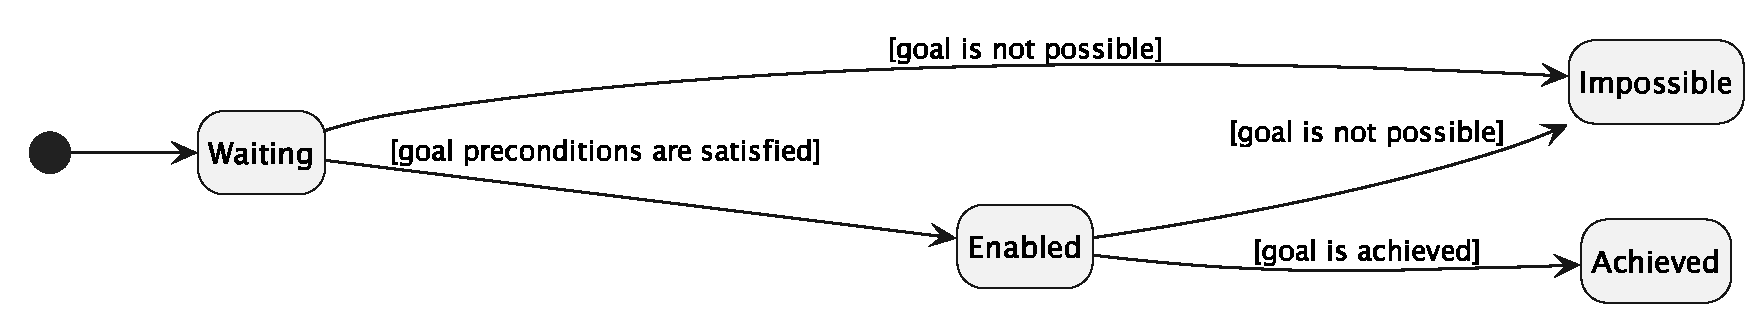
\includegraphics[width=\textwidth]{images/goal-life-cycle.eps}
    \caption{Goal life cycle.}
    \label{fig:goal-life-cycle}
\end{figure}

Each non-leaf goal is decomposed into subgoals by \textit{plans} using three operators:
\begin{itemize}
    \item \textit{sequence}: the plan $g1 = g2, g3$ means that the goal $g1$ is satisfied if and only if $g2$ and subsequently $g3$ are satisfied;
    \item \textit{choice}: the plan $g1 = g2 | g3$ means that the goal $g1$ is satisfied if one and only one of $g2$ or $g3$ is satisfied;
    \item \textit{parallel}: the plan $g1 = g2 \parallel g3$ means that the goal $g1$ is satisfied if both $g2$ and $g3$ are satisfied, and they can be pursued in parallel.
\end{itemize}
Therefore, a social plan denotes a structure of interrelated organizational goals to be satisfied by multiple agents that have to coordinate to handle dependencies between goals.


Goals can be gathered together in \textit{missions}, meaning that they should be achieved under the responsibility of a single agent.
When an agent participates in the organization, it commits to missions, meaning that it will try to achieve the goals contained in them.

All of the above concepts regarding functional abstractions make up a \textit{social scheme}, which denotes the collective and coordinated behavior that is expected to be produced by a group of agents in the organization.

\subsection{Normative Dimension}
Whereas structural abstractions address the structuring of the agents in the system and functional abstractions target the coordination of their behavior, normative abstractions are concerned with the regulation of agents' behavior in the organization

The main concept is the \textit{norm}, which defines the rights and duties of agents by connecting the structural and the normative dimensions with deontic modalities such as \textit{obligation}, \textit{permission}.
Specifically, a norm refers to a role and a mission, thus obliging or permitting the agent playing the role to commit to the mission.
Moreover, a norm can be associated with an \textit{activation condition} that must be satisfied in order for the norm to be active, and a \textit{time constraint} that defines a deadline by which the norm must be satisfied.

\subsection{Organization Execution}
As introduced in \cref{moiseplus}, the organization entity is a representation of the state of the organization at runtime which is distributed into three types of entities.
The concept is similar to the one of \textit{classes} and \textit{objects} in object-oriented programming.

The \textit{group entity} is related to a group defined in the structural specification and its state contains:
\begin{itemize}
    \item the owner of the group;
    \item the links to children and parent groups;
    \item the set of role-player agents with their links.
\end{itemize}

The \textit{scheme entity} is related to a social scheme defined in the functional specification, including:
\begin{itemize}
    \item the owner of the scheme;
    \item the groups responsible for the scheme;
    \item the commitments of the agents to the missions;
    \item the state of each goal.
\end{itemize}

Finally, the \textit{normative entity} is related to group and social scheme entities.
It is created every time a group entity becomes responsible for a scheme entity and it contains the status of a set of norms build from the abstract norms of the normative specification.

\section{Functional Requirements}
Since the platform needs to be compatible with \moise{}, its features should be available in the new platform as well.

\paragraph{Structure}{
    Users should be able to define the structure of the organization.
    In particular, the abstractions that allow its definition are the roles that agents can play, the groups that can contain roles and possibly nest other subgroups, and the links between roles.
    As far as the links are concerned, the core subset of \moise{} should be supported, i.e. extension and compatibility.
}

\paragraph{Behavior}{
    Users should be able to define the expected behavior of the agents.
    Specifically, they will be provided with a way to define the collective goals that agents should achieve and the dependencies among them.
    The type of dependencies supported is \textit{finish-to-start}, meaning that the target goal cannot be pursued until the source goal is achieved.
}

\paragraph{Goal Assignment}{
    Users should be able to assign collective goals to roles, thus connecting the structure and the behavior of the organization.
    Either one, more, or no role can be assigned to a goal and the assignment may have a \textit{obligation} or \textit{permission} deontic modality.
}

\paragraph{Persistence}{
    Users should be able to save and load the organizations they create for future editing.
    Indeed, the platform will provide a way to edit organizations previously created since defining one usually requires multiple iterations and changes.
}

\paragraph{Deployment}{
    Users should be able to enforce the organization they create on running agents.
    In particular, they will choose the agents that will be part of the organization and the roles they will play.
}

\section{Non-Functional Requirements}
Given the target user of this platform, i.e. domain experts, the main non-functional requirement is the ease of use and user-friendliness.
In particular, the interface should be as clean as possible with a minimal set of easy-to-understand features so that users will not feel overwhelmed by it.

What is more, the system should be easily accessible.
Therefore, the most suitable technologies for its development are web-based ones, which allow the user to access the platform from any device with an internet connection.
Although, a mobile version is not required since it will mainly be used on wide screens.

The above functional and non-functional requirements, that arose from the \textit{IntellIoT} project and the need to address a higher level of abstraction for the definition of organization-centered MAS by domain experts, will be therefore fulfilled through the development of a visual programming language and a web-based integrated development environment that exploits it.
\chapter{Design}\label{design}

The following chapter describes the details concerning the design process of the system.

The whole process was carried out with a step-by-step approach, starting from the design of the visual language and early prototypes of the development environment, proceeding with the storage backend, and finally concluding with the integration with the execution backend.

Specifically, the design of the visual language and the development of the web-based IDE prototypes were carried out iteratively, in order to adopt a PDCA (Plan-Do-Check-Act) approach.
The latter allowed receiving realistic feedback straight away, thus intercepting potential problems early on and speeding up the entire process.

Due to the hard time constraint of the internship and to obtain ease of use, although sometimes trading off with expressivity, only a core subset of \moise{} features were implemented.
This also implies that the system was not designed as a complete replacement of \moise{}, but rather as a tool to facilitate the use of this technology also by users with no programming skills.

Moreover, as some parts of the system were designed knowing that they might need a full project focused only on them, this project leaves space for future improvements and integrations, such as the implementation of the remaining features and the exploitation of different technologies.

\section{A Visual Language for Organizations}\label{visual-language}
The main challenge in this project is surely the design of a visual language that, on one hand, is expressive enough to represent the organizational structure and the goals of an organization, and, on the other hand, is easy to use and understand by non-technical users.

Since the visual abstractions are the main artifact of the system, the design of the language was the first step of the project and has gone through several iterations, possibly even evolving further in the future thanks to feedback from real users.

\subsection{The Visual Paradigm}
The choice of the most suitable visual paradigm was the first step of the design process since it is crucial to define the overall look and feel of the language.
Indeed, it is of fundamental importance to choose a paradigm that is easy to use, allows the users to easily understand the meaning of the visual abstractions, is coherent with the concepts to represent, and can be easily translated into the actual specification.

Comparing the existing paradigms for visual programming, the most natural choice was the diagram-based paradigm.
Other approaches, even though already proven to be effective in many fields, were not perfectly suitable for this purpose.
For instance, flow-based programming better fits the modeling of the way data must flow during the execution of the program, while block-based programming is more suitable to describe instructions to be executed in an imperative programming style.

On the other hand, the diagram-based paradigm is appropriate to specify the characteristics of a system in a declarative programming fashion, therefore being highly convenient for the definition of an organizational specification.

\subsection{Reference Language}
To facilitate the design of the visual language, it was necessary to study and understand the organization specification language in order to identify the ``building blocks'' that could be used to represent the organizational structure and the goals of an organization.
Since, as already mentioned, the system has \moise{} as a strong constraint and reference, as the organization specifications created should be compliant with it, the \moise{} language was chosen as a reference.

The analysis of the concepts and the syntax of the reference language, to be ported as visual elements, first involved looking at the \moise{} XML metamodel that defines the rules for the organization specification syntax.
A few examples of the main constructs are shown in \cref{lst:xml-metamodel}\footnote{The entire metamodel can be found at \url{https://github.com/moise-lang/moise/blob/master/src/main/resources/xml/os.xsd}}.

As can be observed, a role definition requires the specification of an attribute \texttt{id}, that is the name of the role, and it may specify some roles it extends from through \texttt{extends} children elements.
On the other hand, a goal definition requires the specification of the attributes \texttt{id}, that is the name of the goal, \texttt{ds}, that is the description, etc. and it may specify arguments, dependencies from other goals, and plans, with \texttt{argument}, \texttt{depends-on}, and \texttt{plan} children elements, respectively.

The actual syntax used in the XML organization specification for roles and goals definition can be found in \cref{lst:xml-model}.

\begin{figure}[H]
    \lstinputlisting[language=XML,label={lst:xml-metamodel},caption={\moise{} syntax rules for the XML specification of roles and goals.}]{code/moise-metamodel.xsd}
\end{figure}

\begin{figure}[H]
    \lstinputlisting[language=XML,label={lst:xml-model},caption={\moise{} actual sintax for the XML specification of roles and goals.}]{code/moise-model.xml}
\end{figure}

\subsection{Organization Structure}
\subsection{Collective Goals}
\subsection{Goals Allocation}

\section{Main Components}
\subsection{Web-Based IDE}
\subsection{Storage Backend}

\chapter{Development}

\subsection{Web IDE}
\subsection{Backend and Specifications Storage}
\subsection{Running Organization Entities}

\chapter{Evaluation}

\section{Case Study - Smart Farming}
\section{Outcome Analysis}

\chapter*{Conclusions}
\addcontentsline{toc}{chapter}{Conclusions}
\markboth{CONCLUSIONS}{CONCLUSIONS}

Qui il testo delle conclusioni alla tesi. Non deve essere un riepilogo di quanto fatto nella tesi ma piuttosto le conclusioni raggiunte relative al lavoro svolto.	
\chapter*{Acknowledgments}
\addcontentsline{toc}{chapter}{Acknowledgments}
\markboth{ACKNOWLEDGMENTS}{ACKNOWLEDGMENTS}

Qualora lo si desideri è possibile inserire qui il testo dei ringraziamenti alle persone che hanno contribuito in qualche modo al percorso che ha portato al lavoro di tesi.
	
\backmatter	

\bibliography{bibliography}{}
\bibliographystyle{plain}

\end{document}